Aussi connu sous le nom  de \emph{théorème de \textsc{Stone-Weierstrass}}

\begin{theo}
    Toute fonction continue sur un segment $[a, b]$ de $\R$ à valeurs dans $\R$ ou $\C$ est limite uniforme sur $[a, b]$ d'une suite de polynômes.
\end{theo}

\begin{preuve}
    \cite{calcul_infinitesimal} page 157.
\end{preuve} 

L'exercice suivant montre qu'il existe une suite de polynômes $(P_n)$ qui converge uniformément vers la fonction racine carrée sur $[0, 1]$.

\begin{exercice}
    \emph{Exercice 5. TD Ch. VIII}\\
    Soit la suite de fonctions définie pour tout $x \in [0, 1]$ par
    $$
    \begin{cases}
        P_0(x) &= 0,\\
        P_{n+1}(x) &= P_n (x) + \frac{1}{2} \big( x-P_n (x)^2 \big).
    \end{cases}
    $$
    Montrer que $(P_n)$ converge uniformément vers une fonction $f$ sur $[0, 1]$.
\end{exercice}

\begin{marginfigure}[-5cm]
	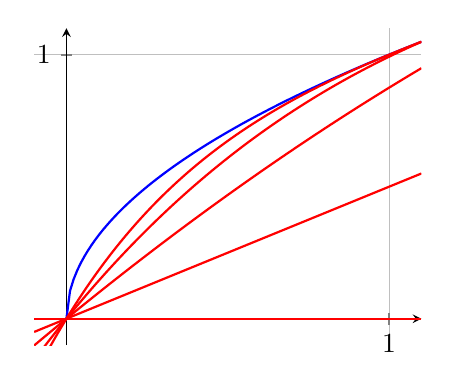
\begin{tikzpicture}
    \begin{axis}[width=6.5cm,
        axis lines=middle,
        grid=major,
        xmin=-0.1, xmax=1.1,
        ymin=-0.1, ymax=1.1,
        % xlabel=$x$, xlabel style={right},
        % ylabel=$y$, ylabel style={above},
        tick style={thick},
        ticklabel style={font=\normalsize},
        xtick={0, 1}, 
        ytick={0, 1},
        % legend entries={0.5x},
            legend style={
            at={(1.05,0.4)},
            anchor=north,
            legend columns=1},
            legend cell align={left}
    ]
    
    \def\a{-0.1}
    \def\b{1.1}
    
    \addplot[blue,thick,samples=100,domain=0:\b] {x^(1/2)} node (racine) {};
    %\node [left] at (racine) {$\sqrt{x}$};
    
    \addplot[red,thick,samples=100,domain=\a:\b] {0} node (P0) {};
    %\node [left] at (P0) {$P_0$};
    
    \addplot[red,thick,samples=100,domain=\a:\b] {x/2} node (P1) {};
    %\node [anchor=north east] at (P1) {$P_1$};
    
    \addplot[red,thick,samples=100,domain=\a:\b] {-1/8*x^2+x} node (P2) {};
    %\node [left] at (P2) {$P_2$};
    
    \addplot[red,thick,samples=100,domain=\a:\b] {-1/128*x^4+1/8*x^3-5/8*x^2+3/2*x} node (P3) {};
    %s\node [left] at (P3) {$P_3$};
    
    \addplot[red,thick,samples=100,domain=\a:\b] {-1/128*x^4+1/8*x^3-5/8*x^2+3/2*x + 1/2*(x-(-1/128*x^4+1/8*x^3-5/8*x^2+3/2*x)^2)} node (P4) {};
    \end{axis}
\end{tikzpicture}


%import matplotlib.pyplot as plt
%import numpy as np
%from numpy.polynomial import Polynomial

%PAS = 1e-3
%n = 8
%X = np.arange(0, 1, PAS)


%P = Polynomial([0])
%plt.plot(X, P(X))

%for k in range(n):
%    P = P + 1/2 * (Polynomial([0, 1]) - P ** 2)
%    plt.plot(X, P(X))

%racine = [np.sqrt(x) for x in X]
%plt.plot(X, racine, 'r')
%plt.show()

\end{marginfigure}

Peut-on génraliser à $\R$ ? \dots

\begin{tcolorbox}
    Si $(P_n)_{n \in \N}$ est une suite de polynômes convergeant uniformément sur $\R$ vers une fonction $f$, alors $f$ est un polynôme.
\end{tcolorbox}

\begin{preuve}
    Source : \cite{exos_oraux} \& \cite{maths-france}. \\
    Soit $(P_n)_{n \in \N}$ une suite de polynômes convergeant uniformément sur $\R$ vers une fonction $f$. \\
    D'après la critère de \textsc{Cauchy} uniforme, il existe un rang $n$ tel que pour tout $p \in \N$, 
    $$\Ninf{P_{n+p} - P_n} \leqslant 1.$$
    La fonction polynomiale $P_{n+p} - P_n$ est donc bornée sur $\R$ autrement dit elle est constante. On a alors,
    $$\forall (p, x) \in \N \times \R,\ P_{n+p}(x) = P_n(x) + P_{n+p}(0) - P_n(0) \xrightarrow[p \to + \infty]{} P_n(x) + f(0) - P_n(0)$$
    donc par unicité de la limite simple, $f : x \mapsto P_n(x) + f(0) - P_n(0)$, qui définit bien une fonction polynomiale. 
\end{preuve}